%\documentclass[conference]{IEEEtran}
\documentclass[draftclsnofoot,journal,onecolumn,11pt]{IEEEtran}

\usepackage{graphicx}
\usepackage{bm}% bold math

\usepackage{epsfig}

%\usepackage{cite}
%\usepackage[bookmarks=true,pdfstartview=FitH]{hyperref}
\usepackage[bookmarks=true,pdfstartview=FitH,,bookmarksopen=true,colorlinks,citecolor=blue,filecolor=green,linkcolor=blue,urlcolor=blue]{hyperref}
\usepackage{bookmark}
\usepackage[cmex10]{amsmath}
\usepackage{algpseudocode}
\usepackage{algorithm}
\usepackage{array}
\usepackage[caption=false]{subfig}
%\usepackage{fixltx2e}
\usepackage{stfloats}
\usepackage{url}
\usepackage{multirow}
\usepackage{threeparttable}

% correct bad hyphenation here
\hyphenation{op-tical net-works semi-conduc-tor}

\begin{document}

\title{On Accurate Measurement of Link Quality in Mobile MIMO-OFDM Systems}
\author{\IEEEauthorblockN{Yongsen MA} \\
\IEEEauthorblockA{Shanghai Jiao Tong University \\
E-mail: mayongsen@gmail.com}
}
\markboth{R\MakeLowercase{esearch} P\MakeLowercase{roposal for} P\MakeLowercase{h}D A\MakeLowercase{pplication of} IE, CUHK}{Yongsen MA}
% make the title area
\maketitle

%\begin{abstract}
%%\boldmath
%The abstract goes here.
%\end{abstract}


\section{Background}

The wireless networks have experienced rapid development in recent years, which leads to the increase of traffic loads and users requirements. The wide expansion of wireless services has brought serious challenges to the issues of spectrum efficiency and required data rate. Recently, WLANs (Wireless Local Area Networks) based on 802.11n have enjoyed tremendous growth due to the ever-increased demands of high-bandwidth applications. Moreover, with the increasing popularity of smartphones, the growth of mobile 802.11n is expected to continue unabated \cite{Bala2010wifi}. On the other hand, the power consumption of wireless communications is becoming increasingly vital to a more efficient and longer lasting mobile battery in mobile wireless systems. The continued success of mobile 802.11n depends on their ability to efficiently configure different PHY/MAC enhancements based on MIMO-OFDM technologies, and here comes the question of how to get energy-efficient trade-off between reliability and data rate in mobile MIMO-OFDM systems?

In order to solve this problem, some approaches on energy-efficient rate adaption have been carried out based on simulations \cite{5510775} \cite{6214414} or experiments \cite{Peng:2011:TPS:2030613.2030628} \cite{Li:2012:ERA:2348543.2348585}. Although these works present different solutions such as convex optimization, packet delivery probing or channel state prediction, they are all based on the information of channel state or link quality. So a basic consideration is the \textbf{accurate channel state estimation and link quality measurement with low overhead}. This is challenging in that multi-configuration in mobile 802.11n not only requires far more samples to acquire sufficient information for all possible channel settings, but also introduces significant complications in channel modeling. Furthermore, channels are more vulnerable to environmental variability and terminal mobility in mobile 802.11n. Therefore, accurate channel measurement and prediction is becoming increasingly important in mobile 802.11n networks.

%
%\subsection{Traffic Requirements}
%\begin{figure}
%\centering
%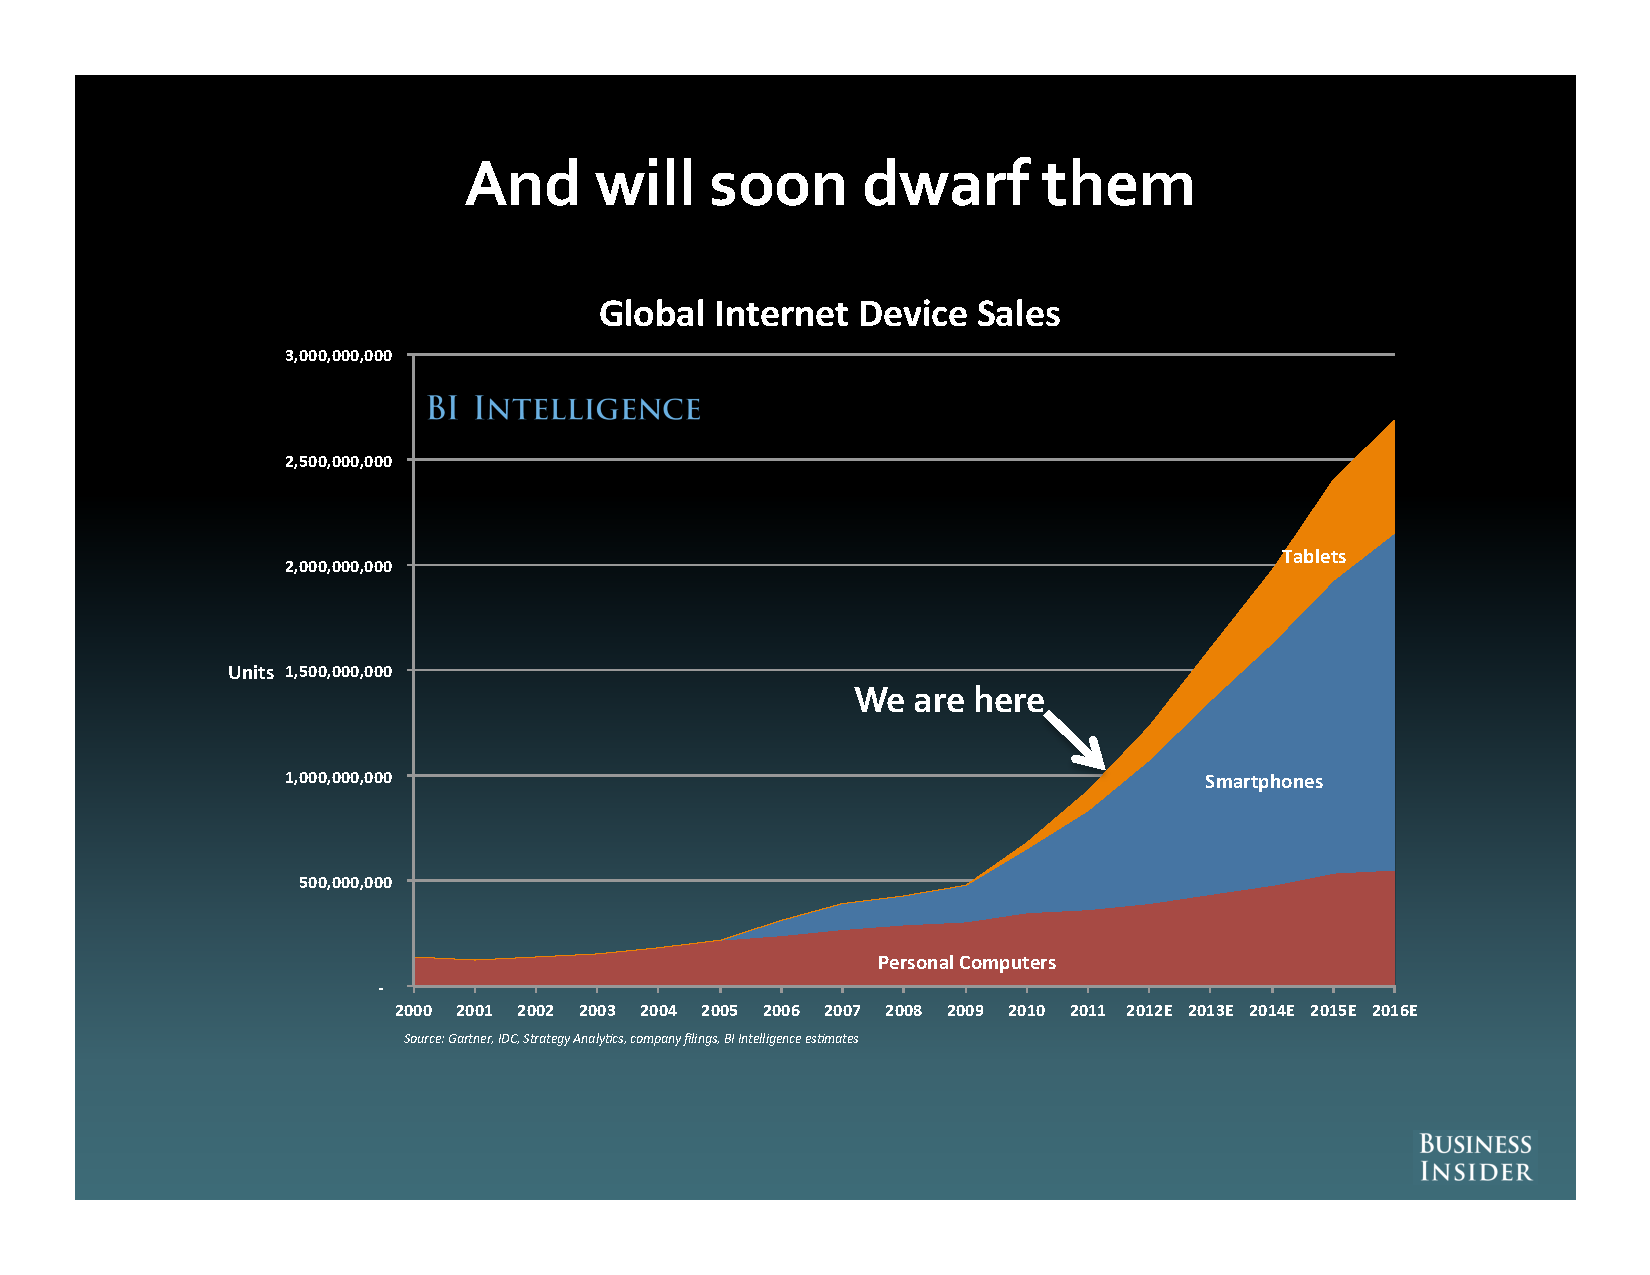
\includegraphics[width=0.8\textwidth]{device_trend.pdf}
%\caption{Global Internet Device Sales.}
%\label{fig:device_trend}
%\end{figure}
%
%\begin{figure}
%\centering
%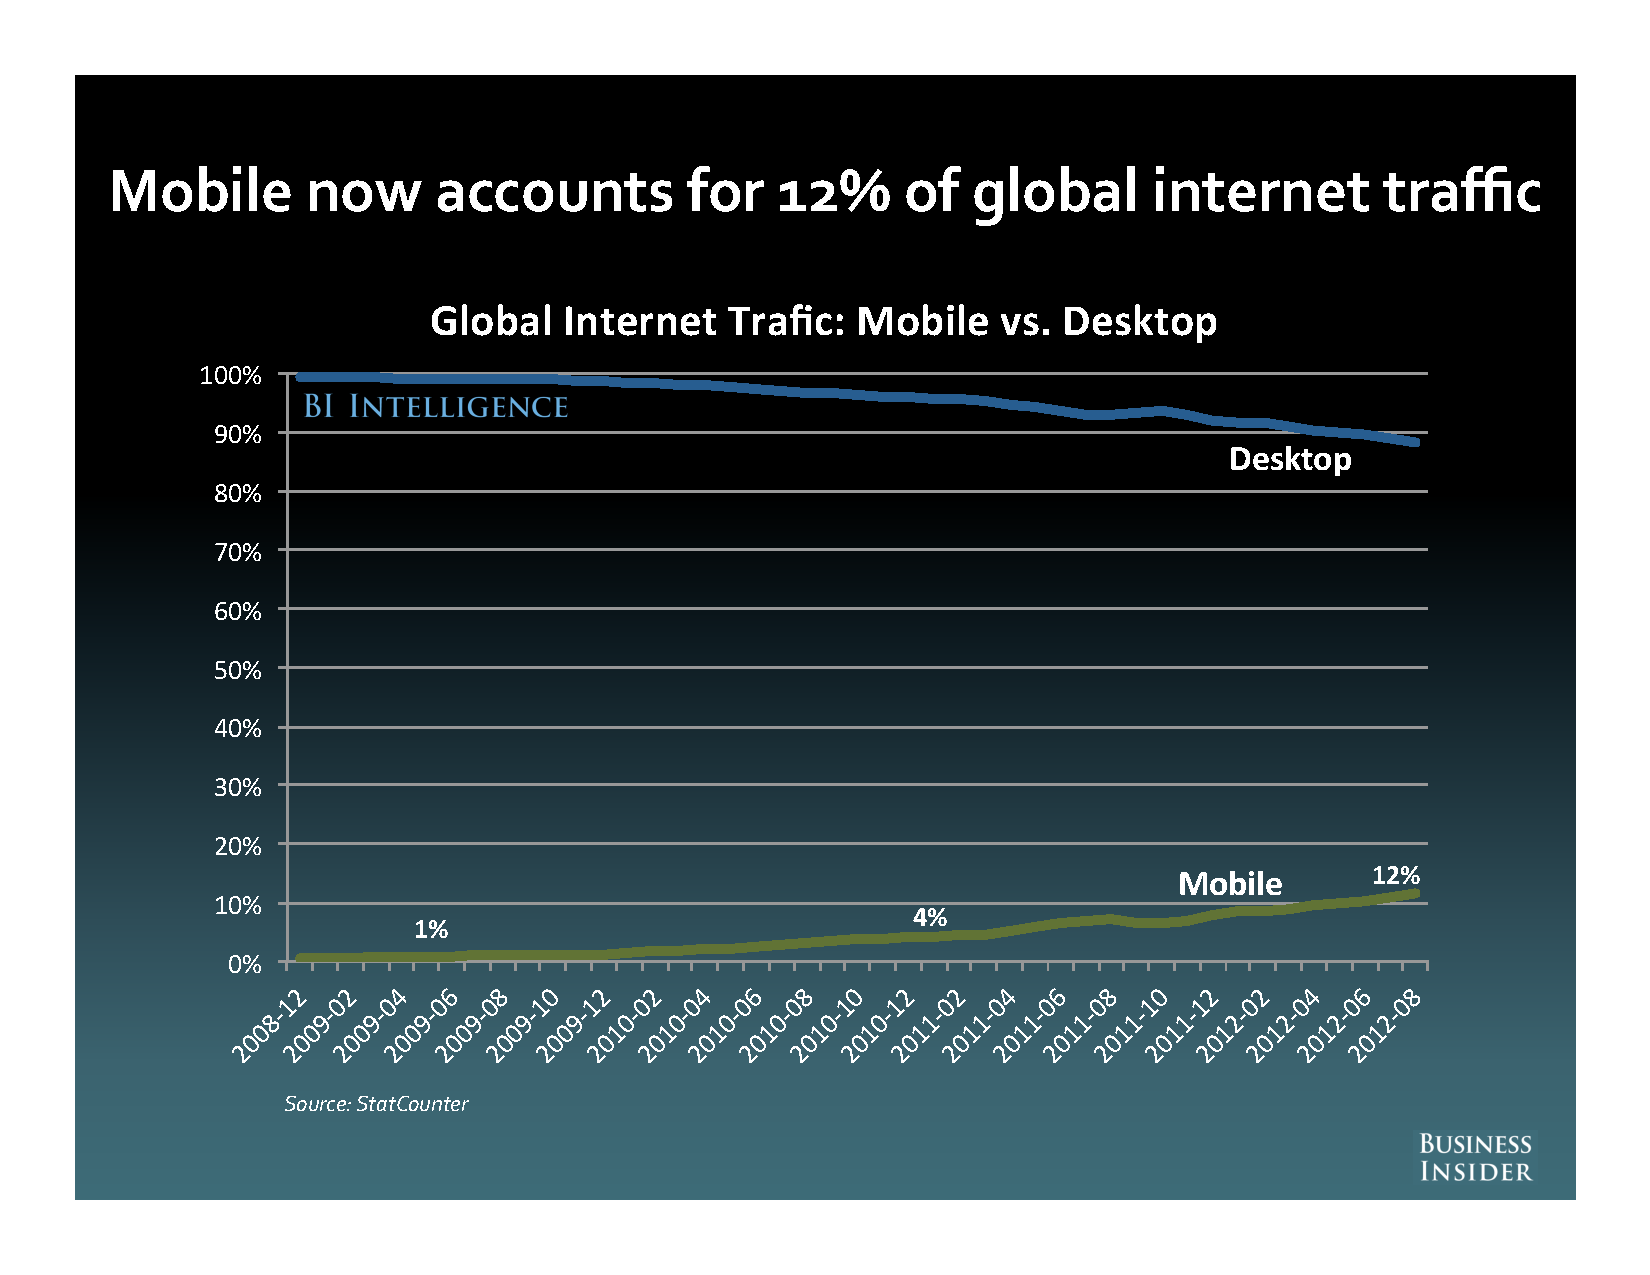
\includegraphics[width=0.8\textwidth]{mobile_desktop.pdf}
%\caption{Global Internet Traffic: Mobile vs. Desktop.}
%\label{fig:mobile_desktop}
%\end{figure}
%
%\begin{figure}
%\centering
%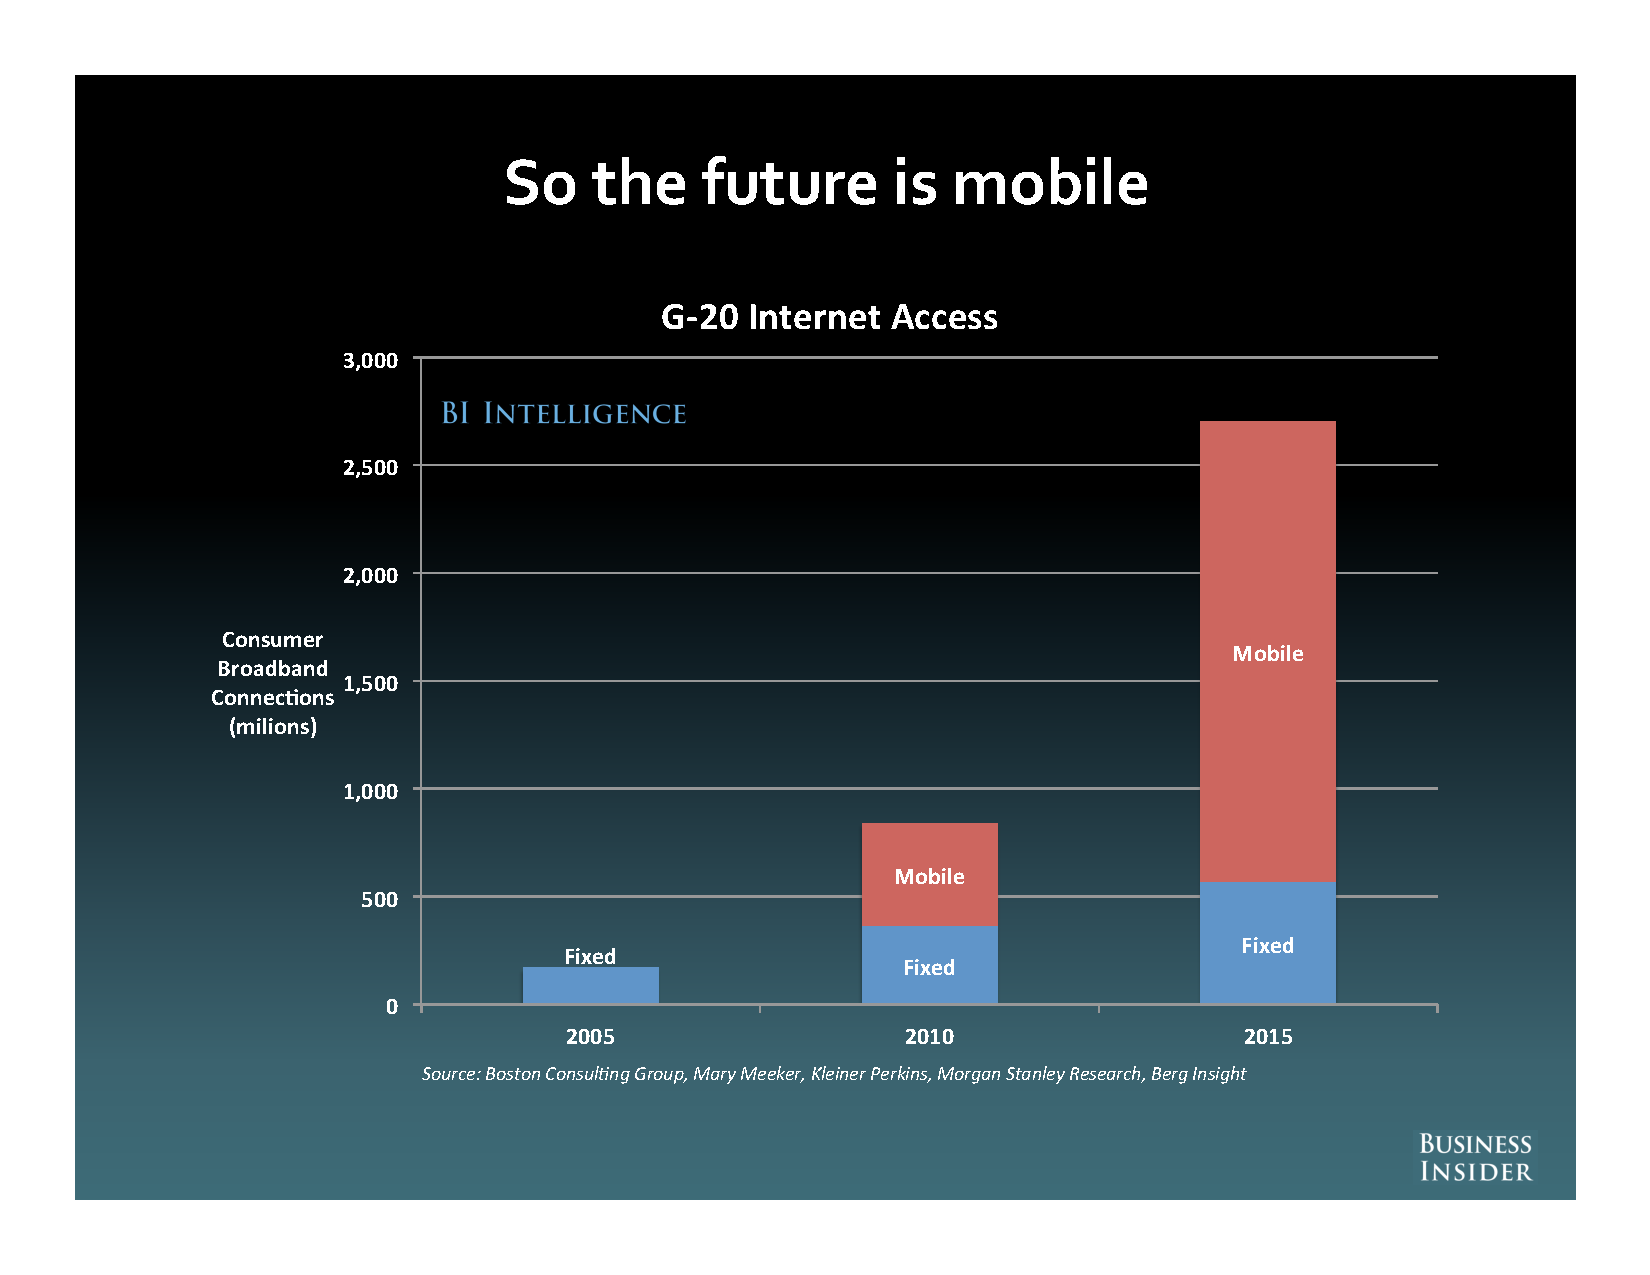
\includegraphics[width=0.8\textwidth]{mobile_trend.pdf}
%\caption{Internet Access: Mobile vs. Fixed.}
%\label{fig:mobile_trend}
%\end{figure}
%
%\begin{figure}
%\centering
%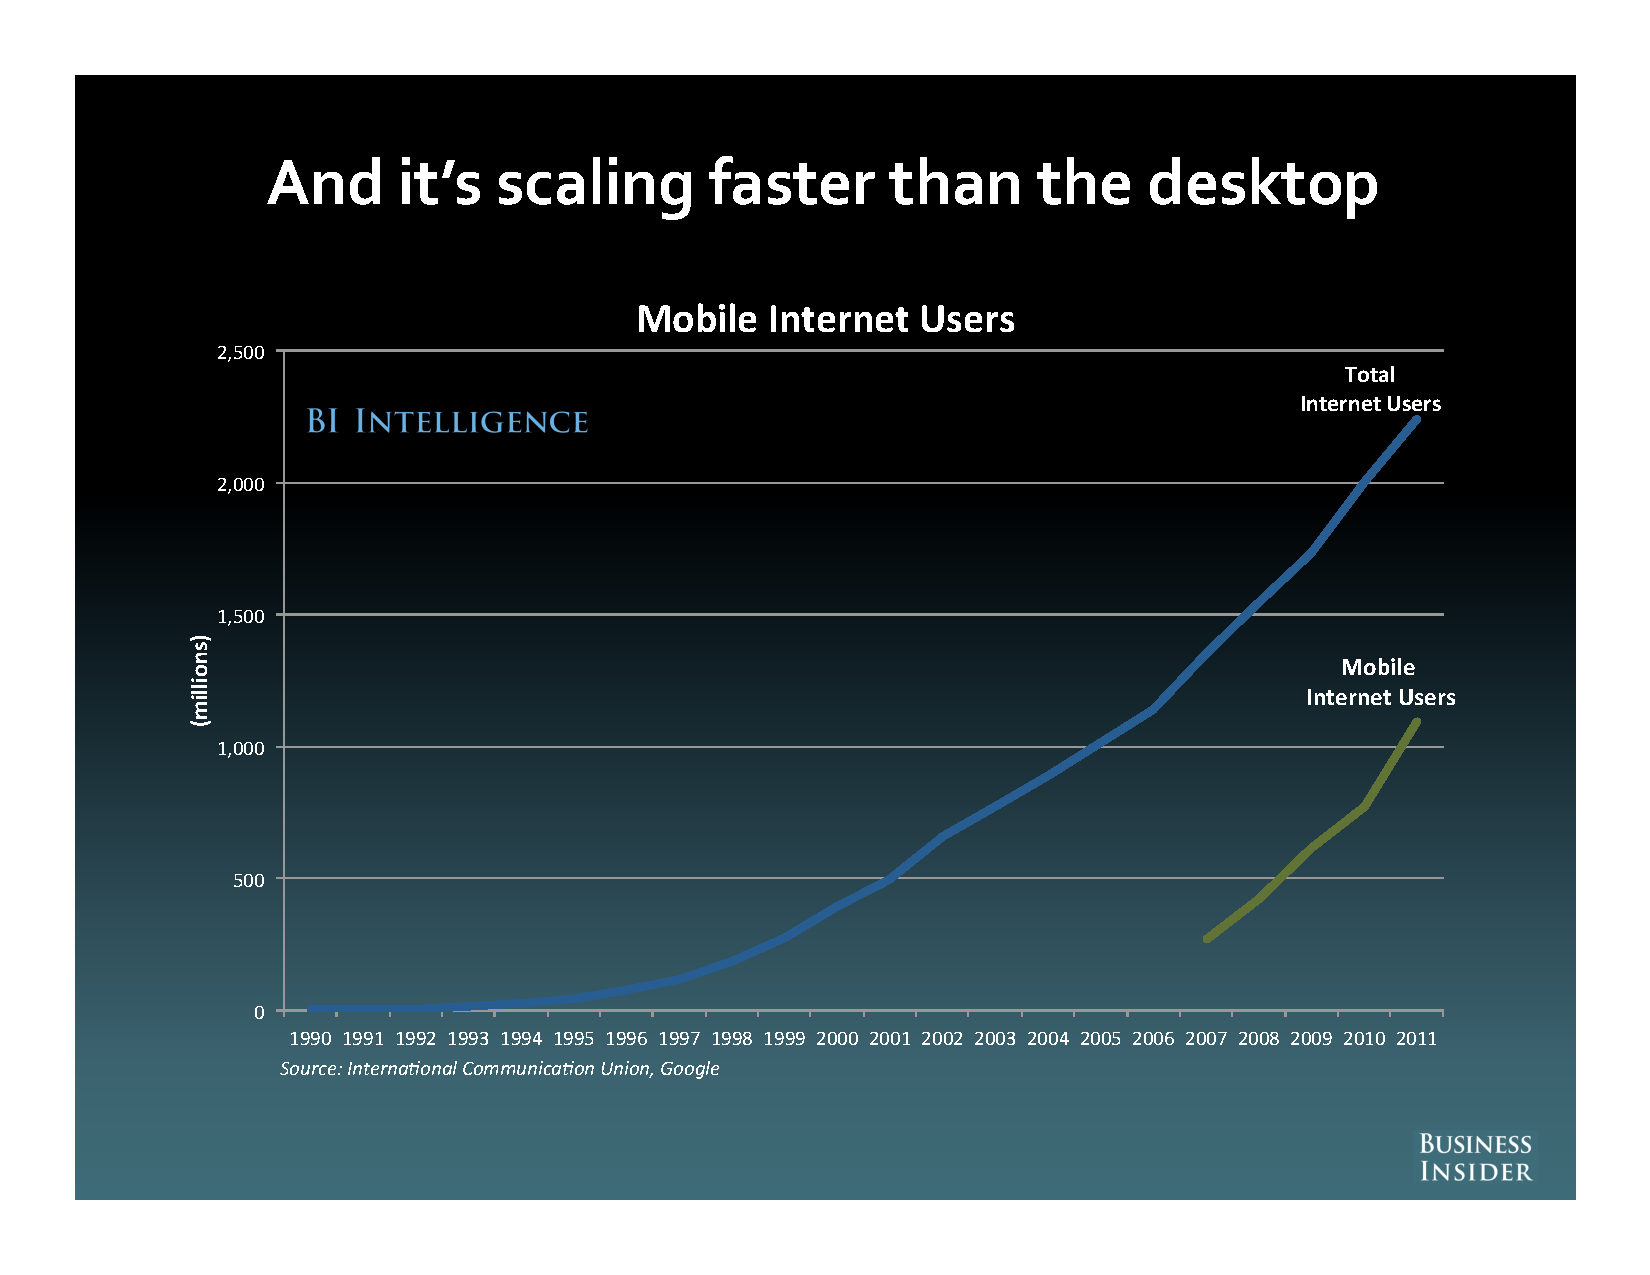
\includegraphics[width=0.8\textwidth]{mobile_users.pdf}
%\caption{Mobile Internet Users.}
%\label{fig:mobile_users}
%\end{figure}
%
%\subsection{Spectrum Efficiency}
%
%\subsection{Energy Efficiency}

\section{Motivations}

The 802.11n standard incorporates PHY/MAC enhancements to achieve higher throughput and wider coverage. In the PHY layer, 802.11n networks adopts MIMO technology to achieve spatial multiplexing and diversity. 802.11n utilizes channel bonding technology, with which two adjacent 20MHz channels are united to a new 40MHz one, to realize higher data rates. In the MAC layer, 802.11n also employs Short Guard Interval (SGI) and frame aggregation to reduce overhead and improve efficiency. All these PHY and MAC enhancements not only play an effective impact on the performance of higher layers, but also make link quality measurement and analysis more complicated. For above configurations of 802.11n, the Packet Delivery Ratio vs. Received Signal Strength (PDR-RSS) model shows different characteristics.

\begin{figure}[!htp]
\centering
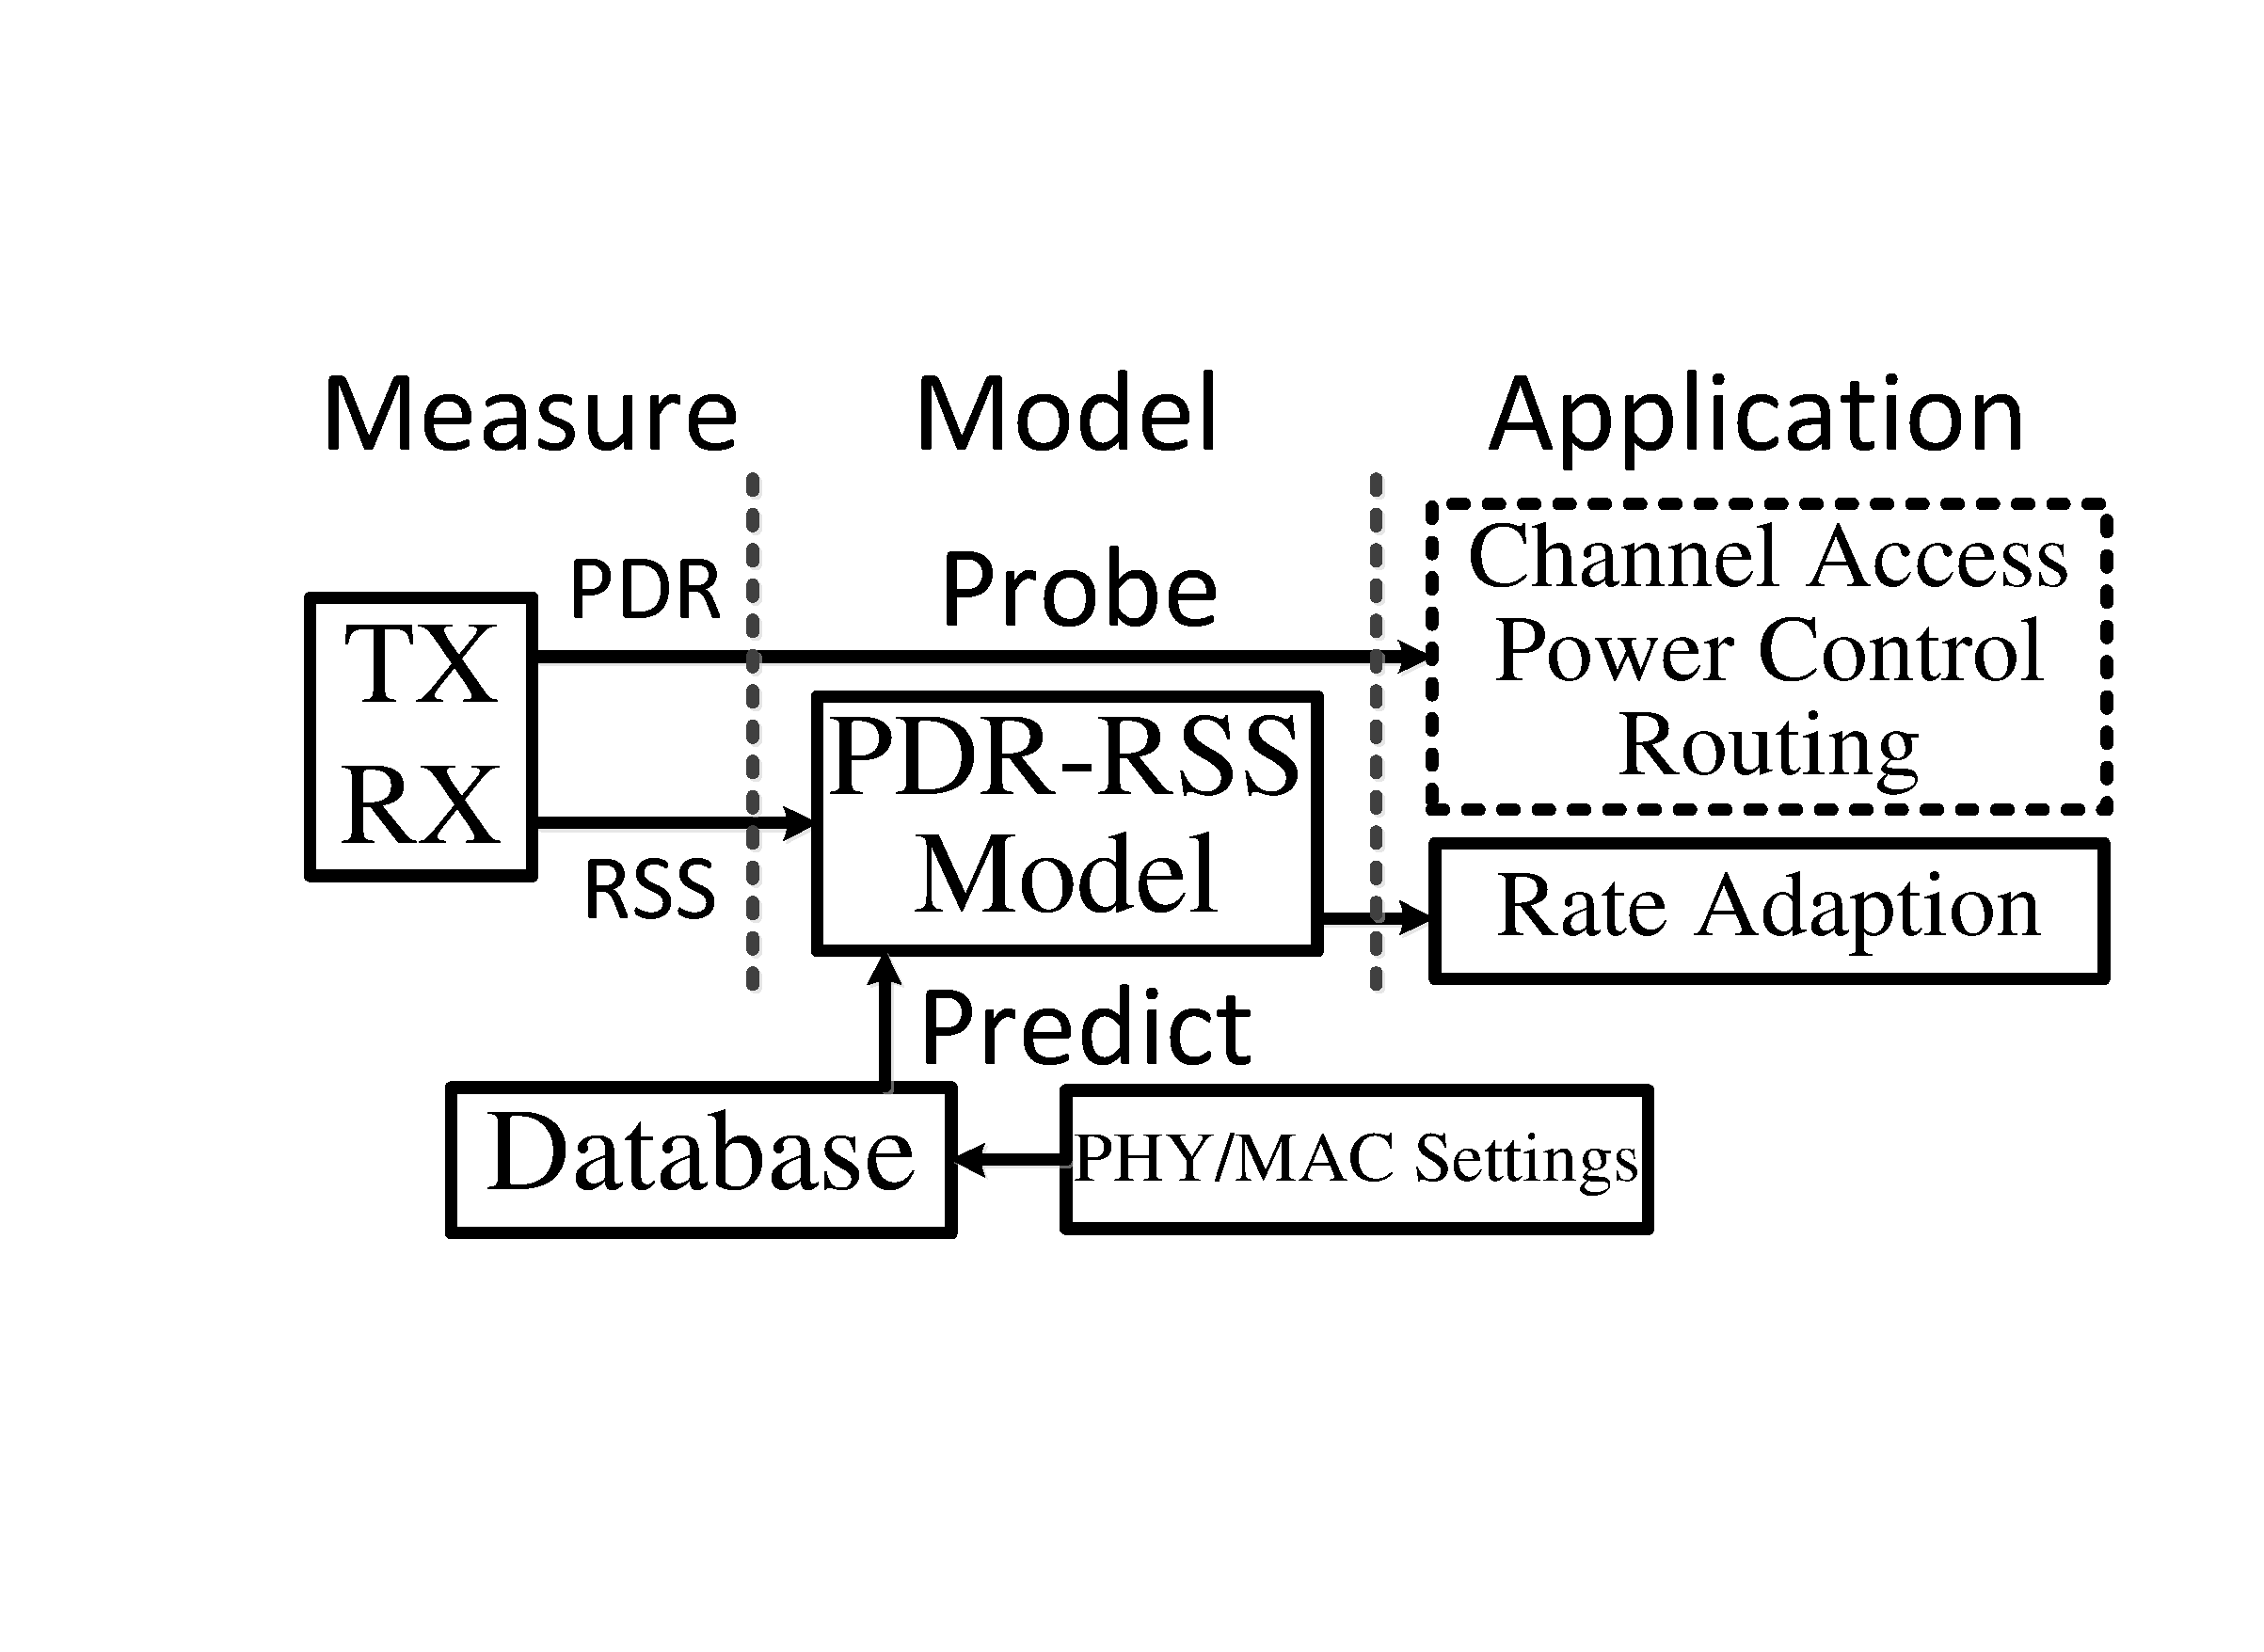
\includegraphics[width=0.5\textwidth]{modeling1.pdf}
\caption{General static PDR-RSS modeling framework.}
\label{offlinemodel}
\end{figure}

The general framework for current channel measurement and prediction methods based on PDR-RSS model is shown in Fig.~\ref{offlinemodel}. The main features in the static framework are as follows:
\begin{enumerate}
  \item static Exponentially Weighted Moving Average (EWMA) for PDR measurement;
  \item static data set and PDR-RSS model;
  \item single measurement metric (PDR or RSS) input.
\end{enumerate}
It will lead to new problems when the static PDR-RSS framework is applied in mobile 802.11n networks, which will be investigated in the following.

\subsection{Time-varying and Location Differences}

\begin{figure}[!htp]
\centerline{
    \subfloat[Time varying]{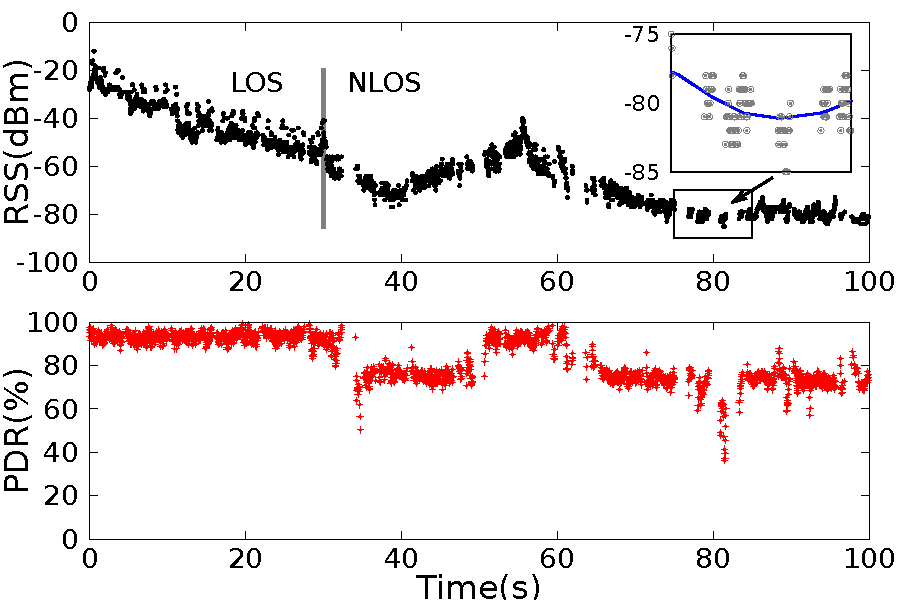
\includegraphics[width=0.4\textwidth]{time.pdf}
    \label{time_vary}
}
    \subfloat[Location difference]{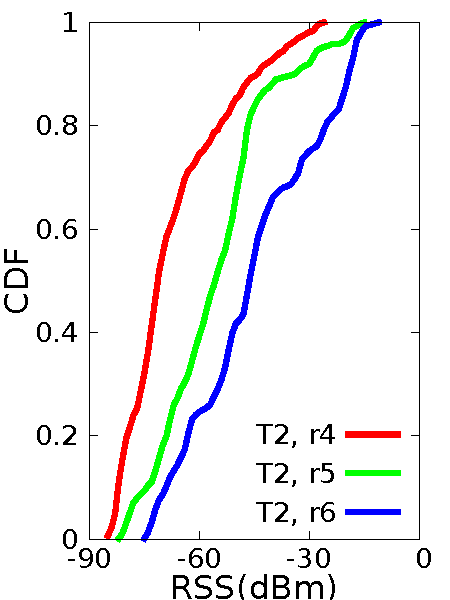
\includegraphics[width=0.2\textwidth]{cdfrss.pdf}
    \label{cdf_rss}
}
    \subfloat[PDR overestimation]{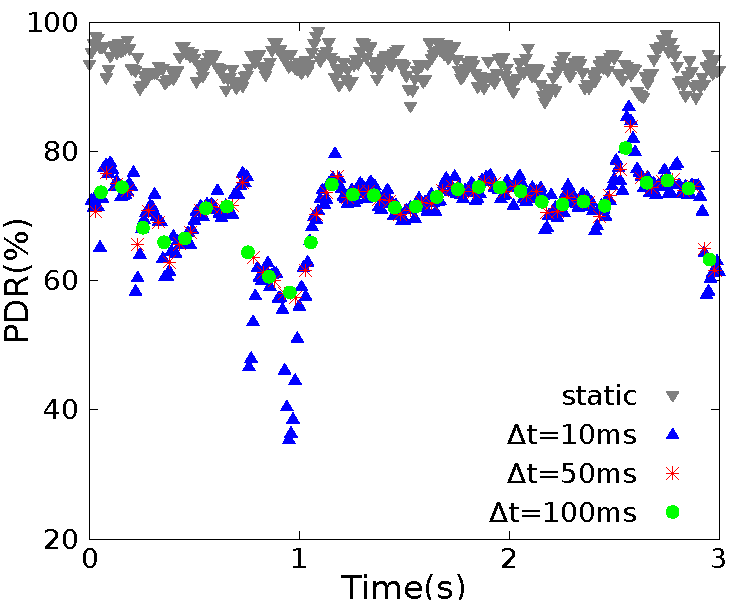
\includegraphics[width=0.333\textwidth]{pdrvary.pdf}
    \label{pdr_over}
}
}
\caption{Characteristics of PDR and RSS in mobile 802.11n, composed of both of LOS and NLOS scenarios.}
\label{time}
\end{figure}

EWMA is widely used in PDR measure \cite{ath9k} \cite{minstrel} \cite{wong2008wireless}, whose sampling interval and weighted factor are both set fixed to 50ms/100ms and 0.125/0.25. However, the time-varying and location difference features of PDR would reduce the measurement accuracy of EWMA, especially when operating at high data rates. The following experiments show that PDR is vulnerable to spatial and temporal diversification in mobile 802.11n networks. RSS and PDR measurements were conducted along different routes by Atheros's 2T2R 802.11n module AR9382 at 5GHz band. Fig.~\ref{time_vary} illustrates that both RSS and PDR encounter with sudden decline in short time scale. The Cumulative Distribution Functions (CDF) of RSS measures with the same 802.11n cards are given in Fig.~\ref{cdf_rss}, which illustrates the location differences of network status. Fig.~\ref{pdr_over} shows a specific measurement example of data rate 78Mbps measured by the same way in Fig.~\ref{time_vary}, where EWMA will overestimate 20\% of PDR when there is a sudden decline. Thus, it is expected to develop dynamic PDR measurement method to increase the accuracy in mobile environments.

\subsection{Transition Windows}
Since 802.11n standard incorporates several enhancements including channel bonding, spatial multiplexing, frame aggregation and SGI, it is a basic problem that how to switch between different operating configurations for better suiting the radio environments. The complexity stems from the large transition windows of PDR-RSS model in 802.11n \cite{Halperin2010predictable}, as shown in Fig.~\ref{fig:pdr}. This situation will be worse when PDR is overestimated by static measurement approach in fast changing channels.

\begin{figure}[!htp]
\centerline{
    \subfloat[PDR-RSS model]{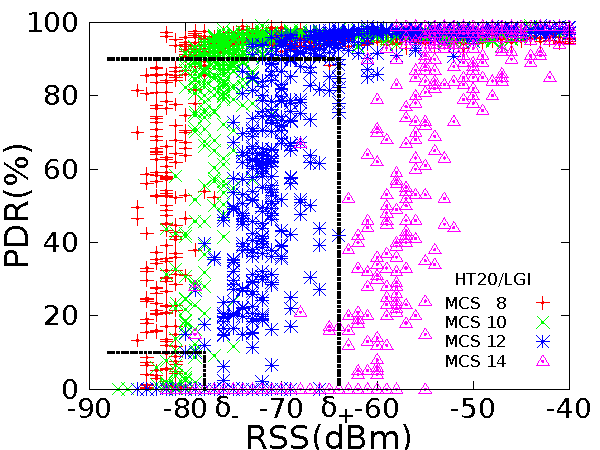
\includegraphics[width=0.4\textwidth]{pdr.pdf}
    \label{fig:pdr}
}
    \subfloat[MCS selection]{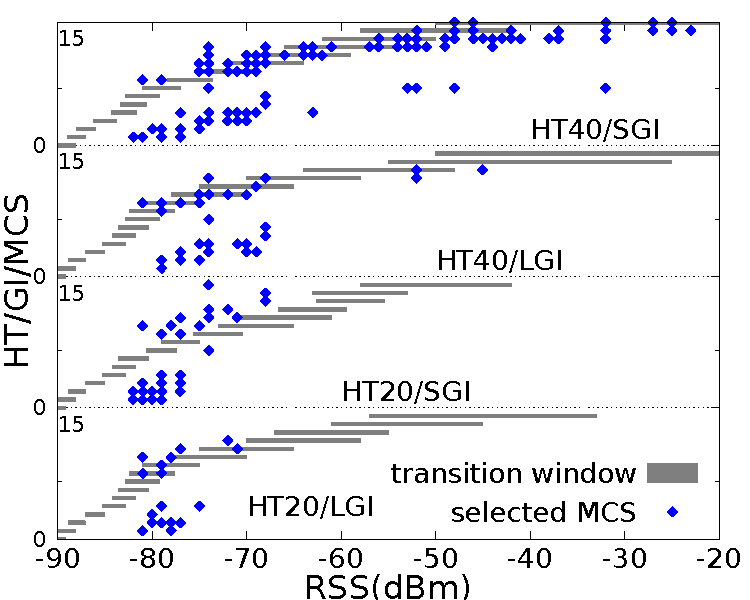
\includegraphics[width=0.38\textwidth]{MCS.pdf}
    \label{MCS}
}
}
\caption{(a) Large transition windows of PDR-RSS model in 802.11n; (b) Large parts of selected HT/GI/MCS fall within the transition window, especially for high data rates.}
\label{pdr-rss}
\end{figure}

Fig.~\ref{MCS} gives an example of rate selection results, which separates the HT/GI/MCS selection and RSS into three regions. The gray lines are the transition windows for each individual HT/GI/MCS selection, and locating just the right of gray line will efficiently improve achieved throughput with high reliability. For every four parts separated by HT/GI options, the selected MCS falling on the right of transition region means it can get high PDR under this setting. There are about 34\% falling into the transition window, and even 8\% are worse that locating on the left of the transition window. However, the good news is that the transition windows exhibit diversity distribution for different MCS selection and channel assignment from Fig.~\ref{MCS}. This indicates that there exists certain configuration(s) for current RSS that can ensure PDR being out of transition window. It provides a hint that we can configure different PHY/MAC enhancements at the right of gray line by jointly utilizing the real-time PDR and RSS, which improves the network throughput with high reliability.

To sum up, 802.11n PHY/MAC enhancements make the PDR measurement and modeling more complicated, and mobile wireless connections are highly changing. These factors significantly reduce the prediction accuracy and rate selection efficiency. The key is to design an on-line PDR-RSS model to address the following issues: (1) high-accuracy PDR measurement; (2) dynamic PDR-RSS model update; (3) efficient configuration(s) output. That is:
\begin{enumerate}
  \item \textit{How to accurately measure PDR with low overhead in fast changing channels?}
  \item \textit{How to characterize the relationship among PDR, RSS and 802.11n multi-configuration?}
  \item \textit{How to update the characterized relationship in real-time and derive the set of configurations with certain reliable performance guaranteeing at current PDR and RSS?}
\end{enumerate}

\section{Literature Review}

\subsection{Related Works}
\subsubsection{Practical Packet Delivery Models}
There are numerous work on practical delivery and interference models. Some early researches paid attention to off-line models in static wireless networks \cite{kolar2011mesh} \cite{reis2006model}, and it is widely used in upper layer applications such as capacity analysis \cite{kashyap2007capacity} and rate control \cite{chen2011ram} \cite{judd2008efficient}. The authors in \cite{10.1109/TMC.2009.87} proposed repeatable measurement in mobile wireless networks that aimed at combining real experiments and simulations. The Sybot in \cite{kim2010sybot} also conducts mobile spectrum survey which only makes RSS measurement but ignore the link level quality. These works are all based on traditional 802.11a/b/g that can not be directly applied in 802.11n networks. A number of studies have investigated the experimental features of 802.11n networks recently \cite{Halperin2010predictable} \cite{k.rayanchu:fluid:}. The authors in \cite{Halperin2010predictable} provided accurate delivery prediction for MIMO-OFDM of 802.11n based on CSI. But the channel estimation of CSI \cite{CSI-SF} requires too much PYH/MAC operations which makes it more complicated for real-time measurement and modeling.

\subsubsection{Rate Adaption}
There are extensively large number of approaches on 802.11n rate control based on simulations or experiments \cite{kim2009experimental} \cite{Pefkianakis:2010} \cite{zhang2008practical}. Some works have been deployed default on Linux platforms, for instance Minstrel \cite{minstrel} for \textit{mac80211} and Atheros for \textit{ath9k} \cite{wong2008wireless}. However, these works are designed for static 802.11 networks, which utilize fixed EWMA calculations to process PDR and spend look around frames to detect available data rates. Some approaches were proposed on rate adaption in mobile environments, but most of them are concentrated on RSS measurement \cite{chen2011ram} \cite{judd2008efficient}. Some upper layer applications such as intrusion detection \cite{5620919} and congestion control \cite{floyd2000equation} employ on-line PDR measurement methods, but the above proposals do not focus on PDR-RSS modeling and rate selection related issues.

Recently, many researchers are working on energy-efficient issues in MIMO-OFDM wireless networks including WiMAX, LTE, WLANS. Some approaches are carried out based on convex optimization \cite{5510775} or CSI probing \cite{6214414} with mathematical analysis and simulations. Others are designed for 3G \cite{Peng:2011:TPS:2030613.2030628} or 802.11n \cite{Li:2012:ERA:2348543.2348585} \cite{Zhang:2011:EEI:2030613.2030637} networks by practical implementation and evaluation. In addition to utilizing physical-layer and packet-layer metrics, some studies aim at automatically adaption algorithm based on traffic patterns of various upper layer applications \cite{Han:2012:DPW:2307636.2307675} \cite{Jang:2011:SEM:2079296.2079308} or users' requirements \cite{Zhuang:2010:IEE:1814433.1814464} \cite{Schulman:2010:BPA:1859995.1860006}. Although these works present different solutions, they are all based on the information of channel state and link quality. Obviously, accurate information of channel state and link quality has significant influence on performance of rate adaption algorithms.

\subsection{Statement of Significance}

The measurement-based PDR-RSS model is widely used for performance analysis in static wireless networks \cite{reis2006model}. It has been successfully exploited in 802.11a/b/g for upper layer applications such as capacity analysis \cite{kashyap2007capacity} and spectrum allocation \cite{k.rayanchu:fluid:}. However, PDR-RSS model exhibits a large transition window in wireless channels due given the fact that the frequency selectivity of the wideband 802.11 channel is not captured by RSS. Halperin \textit{et al.} \cite{Halperin2010predictable} proposed predictable model to determine the subcarrier SNR using CSI and then aggregate into a global metric called eSNR, which provided better characterization for link quality. But CSI-based measurement in 802.11n can dramatically increase the complexity of channel estimation and modeling. Furthermore, commonly used 802.11n wireless devices only provide CSI reports for unicast packets, which clearly affect the efficiency of collecting CSI matrices. Hence, the tradeoff exists between measurement overhead and accuracy which is worthy to be explored, especially in mobile environments.

Prior works on the PDR-RSS modeling are mostly static \cite{kashyap2007capacity} \cite{kolar2011mesh} \cite{reis2006model}. Moreover, a single measurement metric, either packet-level (PDR) or physical-level (RSS), is utilized by upper layer applications\cite{judd2008efficient} \cite{zhang2008practical}. The PDR-RSS model can overcome the channel quality capturing problem if PDR and RSS are jointly considered. This is further supported by exploiting the multi-configuration properties in 802.11n, in which the transition window exhibits diversity distribution for different configurations from our extensive experiments. It indicates that there exists certain configuration(s) for current RSS that can ensure PDR being out of transition windows. This key observation leads to the requirement of on-line PDR-RSS modeling framework, which utilizes real-time PDR and RSS to update PDR-RSS model dynamically and configure PHY/MAC settings in mobile 802.11n.

\section{Research Methodology}

Through the distinctive features, the on-line PDR-RSS modeling framework can provide a systematic solution for the channel quality capturing problems of static PDR-RSS models.

Fig.~\ref{onlinemodel} presents the on-line PDR-RSS modeling framework, which is composed of three components:
\begin{itemize}
  \item \textbf{Database:} contains the raw data of PDR and RSS along with different 802.11n PHY/MAC settings.
  \item \textbf{PDR-RSS model:} a set of data pair for transition windows' lower and upper bound.
  \item \textbf{HT-GI-MCS index:} the configuration selection sequence.
\end{itemize}

The construction of the online framework is consist of the following three steps. First, the database is initialized through empirical experiments. Second, it will be updated under different settings in realtime operating. Finally, the HT/GI/MCS selection sequence can be generated according to the online PDR-RSS model and current status, which can provide optional HT/GI/MCS sorted in order. Fig.~\ref{framework} shows the software architecture, which is composed of network and device layer components:
\begin{itemize}
  \item \textbf{Network layer:} conducts DSWA calculations to determine averaging intervals and sliding factor, and makes update to get HT-GI-MCS indexes.
  \item \textbf{Device layer:} makes PDR computation and RSS averaging driven by TX/RX events respectively, and selects rate indexes according to network layer results as PDR or RSS lower than certain threshold.
\end{itemize}

\begin{figure}[!htp]
\centerline{
\subfloat[On-line modeling framework]{
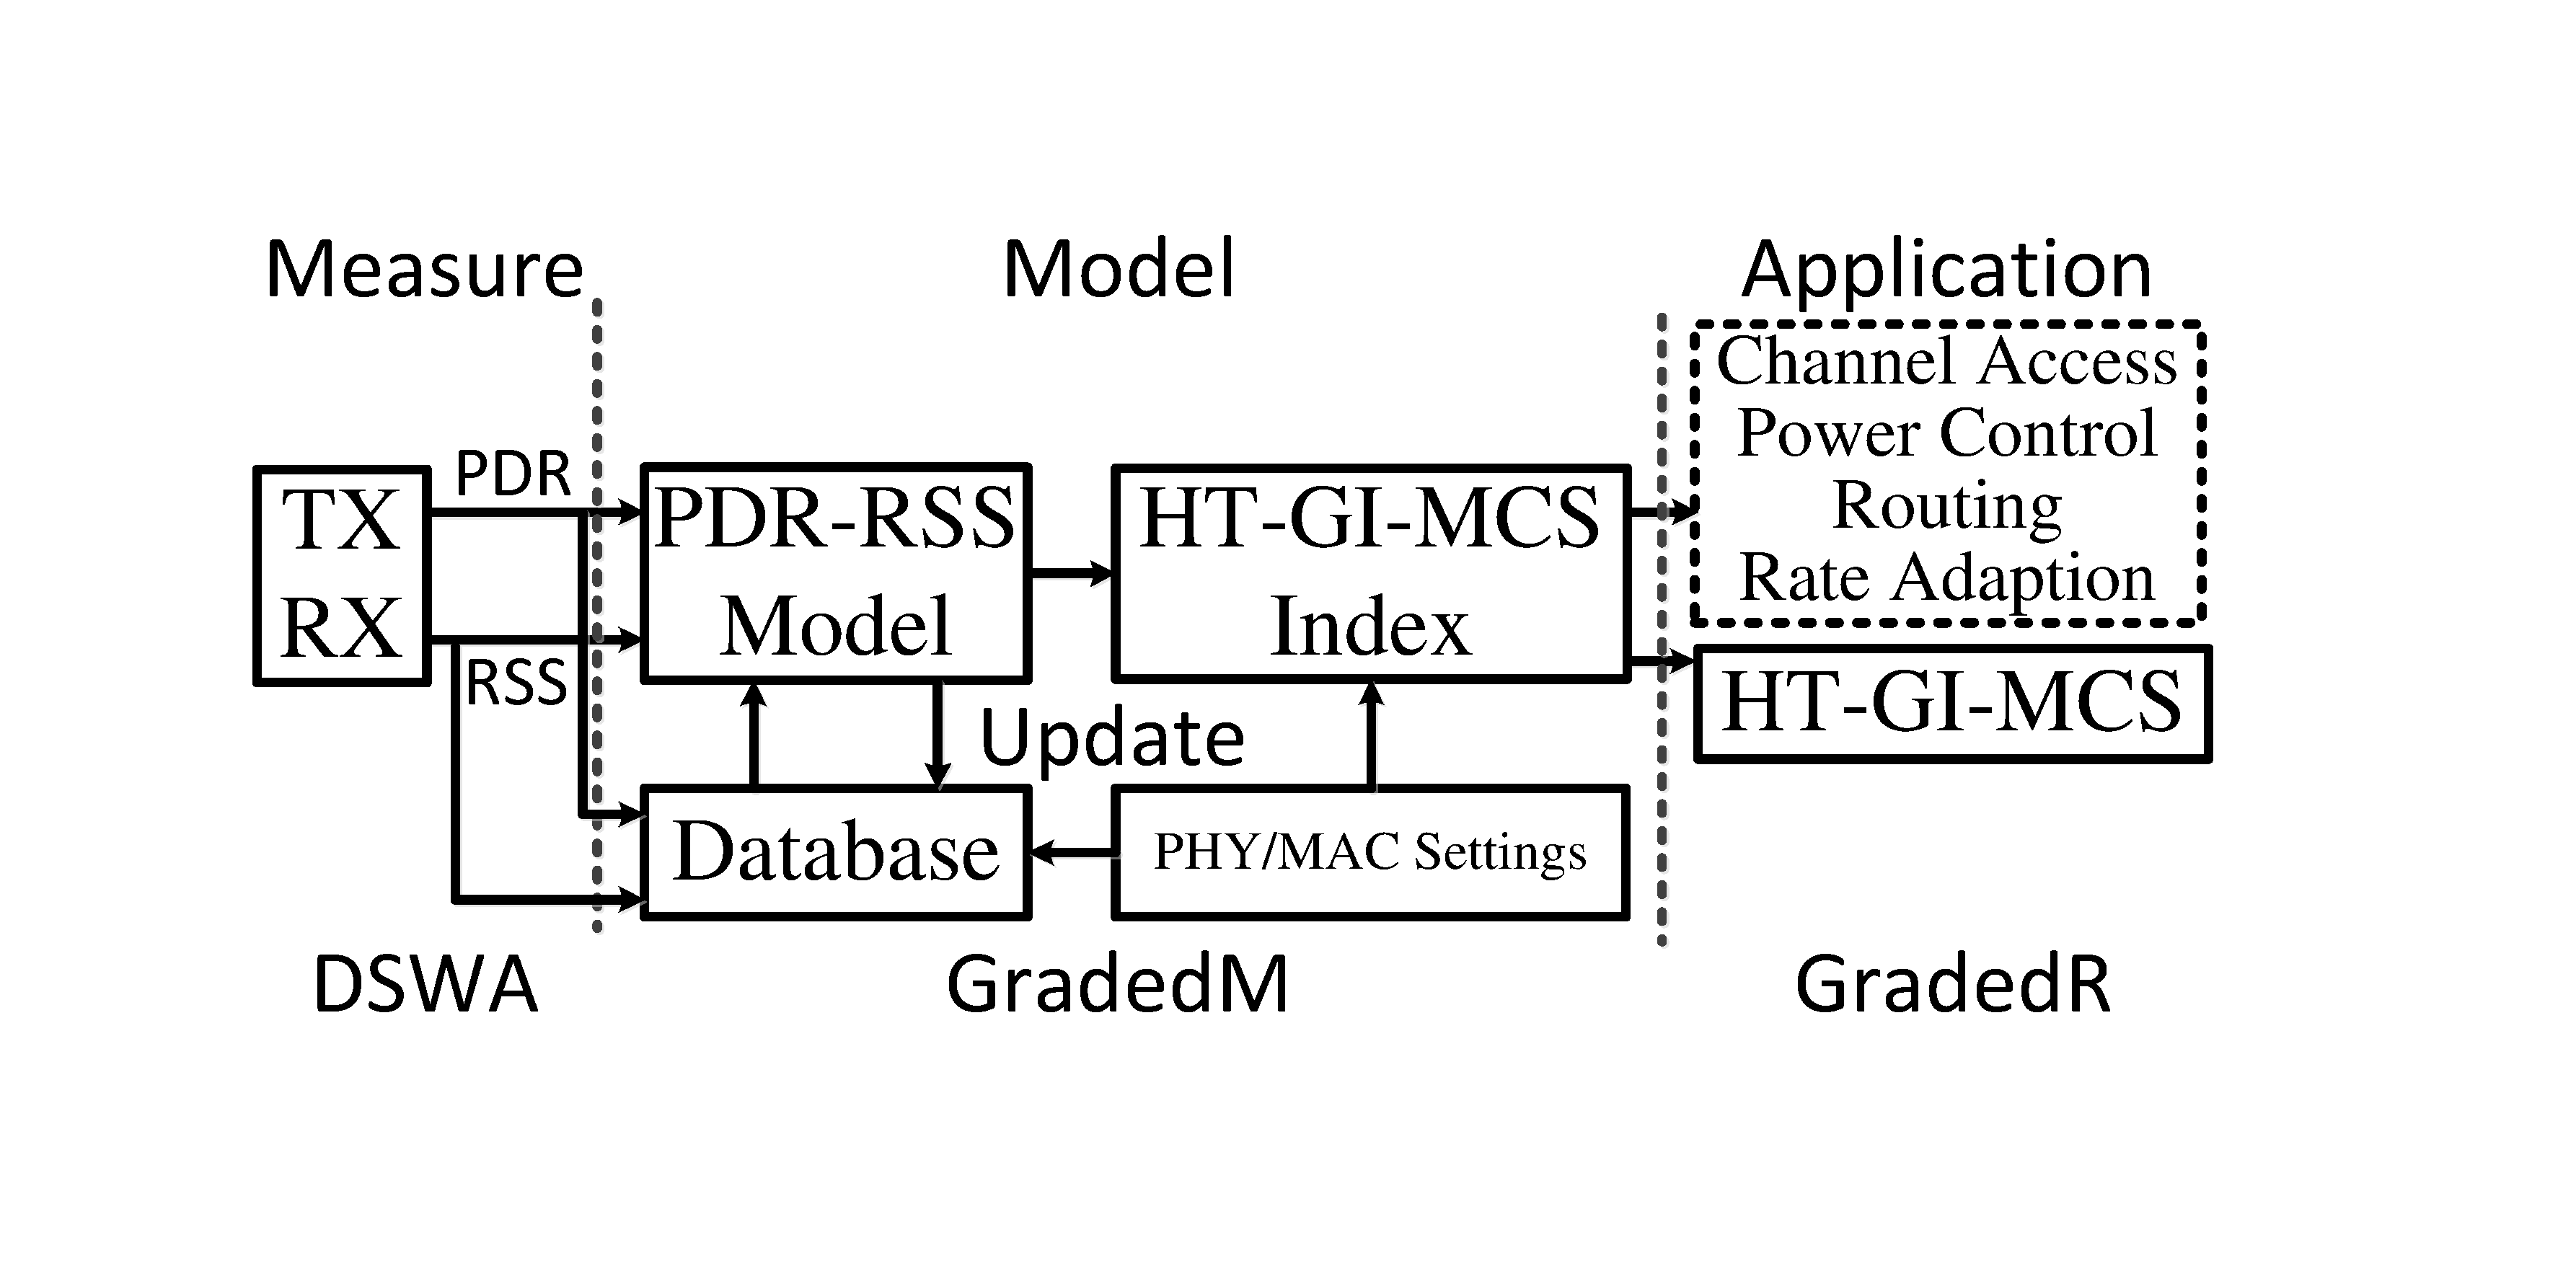
\includegraphics[width=0.55\textwidth]{modeling.pdf}
\label{onlinemodel}
}
\subfloat[Algorithm implementation]{
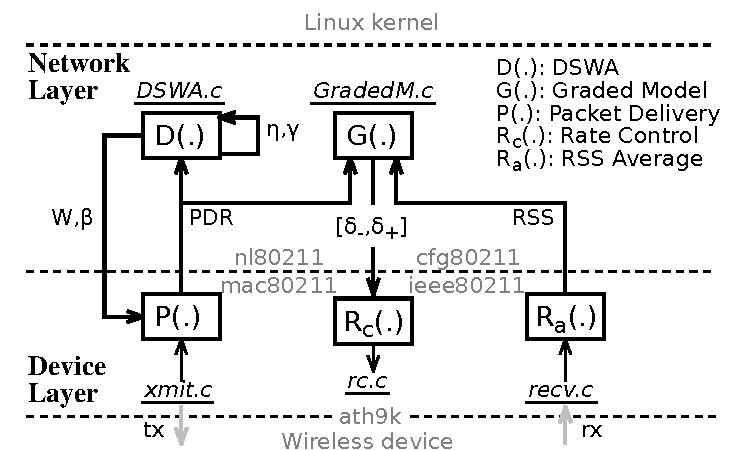
\includegraphics[width=0.45\textwidth]{framework.pdf}
\label{framework}
}
}
\caption{On-line modeling framework and algorithm implementation}
\label{implamentation}
\end{figure}

Compared to the general static PDR-RSS modeling framework in Fig.~\ref{offlinemodel}, the on-line framework has the following distinctive features. First, it has two inputs into both PDR-RSS model and database. Second, both PDR-RSS model and database are updated online. Third, it exploits both real-time PDR and RSS, along with the diversity property to derive the set of configuration(s) with certain reliable performance guaranteeing. In the following, the report gives a thorough design process for the on-line framework to demonstrate how to address the three critical issues: high-accuracy PDR measure, dynamic PDR-RSS model update and efficient configuration output, in the on-line modeling framework.

\subsection{Packet Delivery Measurement} \label{sect:methodology}
For the statistical PDR-RSS model based on realistic measurement in mobile wireless networks, there is a trade-off between measurement accuracy and overhead. The measurement period should be set short enough and responding rapidly to changing network status, or be long cycle to reduce overhead when link quality is steady and reliable. At the same time, both RSS and PDR have time varying and location difference features in mobile 802.11n. And the diversification in data rates and packet size will significantly complicate the programming process. In the traditional rate control algorithms of Atheros's Linux wireless drivers, both \texttt{Madwifi} for 802.11a/b/g and \texttt{ath9k} \cite{ath9k} for 802.11n, EWMA is used to process PDR of each configuration, as shown in Fig.~\ref{weighted}. EWMA has some deficiencies when applied in mobile 802.11n.

\begin{itemize}
  \item The weighting coefficient $\alpha$ is set fixed to 0.125 or 0.25 in practical implementation \cite{ath9k} \cite{minstrel}, and it is hard to respond promptly to link quality changes \cite{EWMAChart}.
  \item The update cycle is also fixed to 50ms or 100ms, which can not achieve effective control on accuracy and overhead. This will lead to PDR overestimation at high data rates as shown in Fig.~\ref{pdr_over}.
\end{itemize}

\begin{figure}[!htp]
\centerline{
\subfloat[EWMA, weighted window]{
    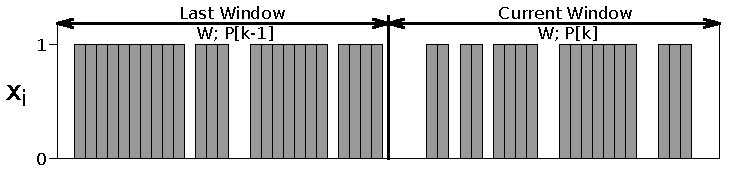
\includegraphics[width=0.5\textwidth]{m_weighted.pdf}
    \label{weighted}
}
%}
%\centerline{
\subfloat[DSWA, sliding window]{
    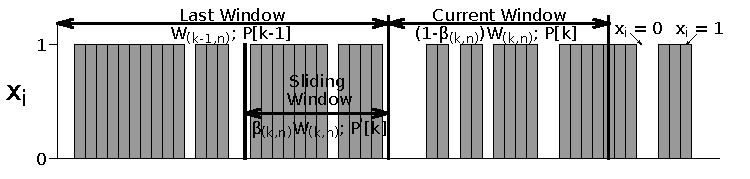
\includegraphics[width=0.5\textwidth]{m_sliding.pdf}
    \label{sliding}
}
}
\caption{Averaging window length in PDR measurement}
\label{method}
\end{figure}

The Dynamic Sliding Window Average (DSWA) approach can be employed to resolve this dilemma. DSWA is event driven and unrelated to data rates, and it takes advantage of sliding window averaging to emphasize on the most recent status. It can be inferred that the measurement errors are closely associated with channel state changes, which have different features in static or mobile wireless networks. Assuming the same average intervals, it will increase the measurement errors when channel state encounters with sudden changes in short time scale.

\subsection{Packet Delivery Modeling} \label{sect:modeling}

PDR is the link layer metric that influenced by physical layer channel state quality, along with antenna numbers, streams, coding and modulation. Moreover, the packet transmission feature is also impacted by traffic loads and users requirements. So on-line PDR-RSS modeling should include these considerations to make effective link adaption according to propagation environments and traffic patterns.

\subsubsection{PHY-layer Channel State}
First, the relationship between PDR and RSS under different MIMO-OFDM configurations should be explored. The on-line PDR-RSS modeling is to update the PDR-RSS database, and generate the HT/GI/MCS sequence according to current network conditions. Obviously, the reliability can be identified by the distance between transition windows' upper bound and current RSS, by wiich the database is sorted in order. Then HT/GI/MCS selection sequence is generated accordingly.

\subsubsection{APP-layer Traffic Patterns}
Second, it has been stated and verified by experiments that traffic patterns have significant influence on packet inter-arrival interval \cite{Han:2012:DPW:2307636.2307675}, network events \cite{Wei:2012:PMP:2348543.2348563} and energy consumption \cite{Mittal:2012:EDE:2348543.2348583}. Thus, the PDR-RSS model can be classified into different categories according to the upper layer traffic patterns. This can be helpful for rate adaption algorithms to make better adjustment to traffic loads and user requirements.

\section{Outcomes and Values}

\subsection{Measurement}
\subsubsection{Accuracy}
For the PDR measurement in realistic networks, EWMA can hardly get sufficient measurement accuracy compared to DSWA. In mobile wireless networks, the propagation environments are complex and communication terminals are on the move particularly, which means both RSS and interference are changing during PDR measurement. This will make PDR changes in short time scale so that EWMA with fixed settings tends to overestimate the actual PDR. Compared with the traditional EWMA method, DSWA will improve the overall measurement accuracy in mobile scenarios.

\subsubsection{Overhead}
In addition to meet the accuracy requirements, it also deserves attention to reduce measurement overhead, since more sample packets will lower the throughput achieved. The averaging intervals of DSWA are associated with PDR changes to allow a more timely response to sustained decreasing in link quality, and make less frequent samples as network conditions are in steady continuously. The averaging window lengths of EWMA are approximately constant for certain rate that $W=20$ for 6.5Mbps and $W=500$ for 300Mbps. When PDR increases and getting stable, DSWA will reduce measurement overhead significantly.

\subsection{Performance}

\subsubsection{Reliability}

DSWA can be adopted to get accurate PDR measurement with low overhead, then the suitable configuration can be chosen according to HT/GI/MCS index. First, DSWA is adaptive to sudden PDR declines to avoid PDR overestimation, which will not lost the information that current PDR is lower that certain threshold. Moreover, when the selected MCS is close to the right bound of its transition window which means the current configuration falls into the transition window, it will reduce the data rate to improve the wireless reliability.

\subsubsection{Throughput}

For the on-line modeling framework, it first adopts DSWA measurement method to get accurate PDR prediction adaptive to network conditions, and then sorts the configuration selection table according to current PDR and RSS. These two procedures not only reduce the measurement overhead but also improve rate selection efficiency, which can improve network throughput effectively. The first aspect is the measurement overhead. Since the on-line framework does not need \lq\lq look around\rq\rq~ frames to gather statistics, it will improve the achieved throughput. The second factor is the measurement accuracy. The on-line framework updates the sensitivity table real-time and chooses the most suitable rate indexes for current conditions, rather than randomly select a lower looked around rate which can hardly meet the current situation and it will increase unnecessary load of wireless link. The achieved PDR can also avoid concussion of network status, when the network conditions are good enough.

\subsection{Energy-efficiency}
There are two kinds of trade-off in mobile MIMO-OFDM wireless systems. The first is the trade-off between reliability and throughput in link adaption based on PHY/MAC configurations, on which the energy-efficient issues are considered by many works recently. Another one is the trade-off between accuracy and overhead for channel state estimation and link quality measurement. Since accurate information of channel state and link quality provides a fundamental guarantee for energy-efficient link adaption, the on-line modeling framework can improve the energy-efficiency of mobile MIMO-OFDM systems.

%\nocite{*}

\renewcommand\refname{References}
%\bibliographystyle{alpha}
\bibliographystyle{apalike}
%\IEEEtriggeratref{6}
\bibliography{wireless}
%\printbibliography

\end{document}
